\documentclass[11pt]{article}
%Gummi|061|=)
\usepackage{amsmath}
\usepackage{amsthm}
\usepackage{amsbsy}
\usepackage{amssymb}
\usepackage{inputenc}
\usepackage{rotating} 
\usepackage{graphicx}
\usepackage{selinput}
\SelectInputMappings{
adieresis={ä},
germandbls={ß},
}
\title{\textbf{Versuch V301: EMK und Innenwiderstand von Spannungsquellen}}
\author{Martin Bieker\\
		Julian Surmann\\
		\\
		Durchgef\"{u}hrt am 28.11.2013\\
		TU Dortmund}
\date{}
\usepackage{graphicx}
\begin{document}
\renewcommand\tablename{Tabelle}
\renewcommand\figurename{Abbildung}
\maketitle
\thispagestyle{empty}
\newpage
\clearpage
\setcounter{page}{1}

\section{Einleitung}
In diesem Versuch sollen die Eigenschaften realer Spannungsquellen betrachtet werden. Von besonderer Bedeutung sind hier die Leerlaufspannung und der Innenwiderstand.
\section{Theorie}
Als Spannungsquelle beschreibt man ein elektrisches Bauteil mit zwei Anschl\"ussen, das zwischen diesen Polen \"uber einen endlichen Zeitraum eine gleichm\"a\ss ige Spannung bereitstellt. Bei einer idealen Spannungsquelle h\"angt diese Spannung nicht von entnommenenem Strom ab.
\begin{figure}[htp]
\centering
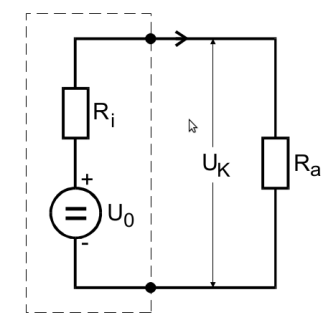
\includegraphics[scale=1.00]{abb3.png}
\caption{Ersatzschaltung f\"ur eine reale Spannungsquelle}
\label{Ersatz}
\end{figure}
Eine reale Spannungsquelle durch eine Ersatzschaltung aus einer idealen Spannungsquelle und einem Widerstand $R_i$ dargestellt werden (siehe Abb. \ref{Ersatz}). Hierbei ist $R_i$ der Innenwiderstand der Quelle und  $U_0$ die sogenannte Leerlaufspannung, dies ist die Spannung, die zwischen den Polen anliegt, wenn aus der Spannungsquelle kein Strom entnommen wird. $U_k$ ist die Klemmenspannung, die zwischen den Polen der belasteten Quelle anliegt. Gem\"a\ss\ der Maschenregel (2. Kirchhoffsches Gesetz)
\begin{equation}
0 = -U_0 + U_k + U_{Ri}
\end{equation}
und dem Ohm'schen Gesetz
\begin{equation}
U_{Ri} = R_i \cdot I
\end{equation}
gilt f\"ur die Klemmenspannung
\begin{equation}
U_k = U_0 - R_i \cdot I.
\label{Klemmenspannung}
\end{equation}
Hieraus folgt, dass die Klemmenspannung einer realen Spannungsquelle bei Belastung kleiner ist als die Leerlaufspannung. Eine ideale Spannungsquelle dagegen hat keinen Innenwiderstand. Desshalb ist die Klemmenspannung in diesem Fall unabh\"angig von der Belastung der Quelle.
Des Weiteren wird aus Gleichung (\ref{Klemmenspannung}) ersichtlich, dass man einer realen Spannungsquelle nur eine begrenzte Leistung $P_{Max}$ entnehmen kann. Aus 
\begin{equation}
P = U \cdot I = R_a \cdot I^2 = \frac{U_0^2 * R_a}{(R_a+R_i)^2}
\end{equation}
folgt f\"ur den Lastwiderstand $R_a$
\begin{equation}
\frac{dP}{dt} = 0 \rightarrow R_a = R_i
\end{equation}
mit einer der maximalen Leistung 
\begin{equation}
P_{Max} = \frac{U_0^2}{4\cdot R_i}.
\end{equation}

\section{Versuchsdurchf\"uhrung}
Im diesen Versuch werden $U_0$ und $R_i$ f\"ur folgende Spannungsquellen bestimmt. 
\begin{itemize}
\item Monozelle
\item RC-Generator (Rechteckspannung)
\item RC-Generator (Sinusspannung)
\end{itemize}
\subsection{Direkte Messung der Leerlaufspannung}
Die Klemmenspannung wird zun\"achst mit einem Voltmeter gemessen. Da dieses einen hohen Eingangswiderstand hat, flie\ss t nur ein geringer Strom und in Formel (\ref{Klemmenspannung}) kann der Term $R_i \cdot I$ vernachl\"assigt werden, sodass gilt: 
\begin{equation}
U_0 \approx U_k.
\end{equation} 

\subsection{Messung an der belasteten Spannungsquelle}
Um den Innenwiderstand $R_i$ und nochmals die Leerlaufspannung $U_0$ zu messen wird die Spannungsquelle ein variabler Lastwiderstand $R_a$ angeschlossen und die Klemmensapnnung $U_k$ sowie der entnommene Strom $I$ gemessen. Abbildung \ref{Aufbau1} zeigt den verwendeten Aufbau. 
\begin{figure}[htp]
\centering
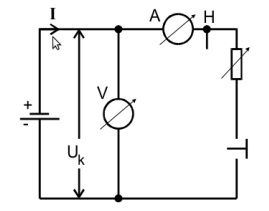
\includegraphics[scale=1.00]{abb1.png}
\caption{Versuchsaufbau ohne Gegenspannung}
\label{Aufbau1}
\end{figure}
Die Gr\"o\ss e des Lastwiderstandes wird gleichm\"a\ss ig in den folgenden Bereichen variiert:
\begin{table}[h!]
\centering
\begin{tabular}{|c|c|c|}
\hline
Spannungsquelle& $R_{Min} [\Omega]$& $R_{Max} [\Omega]$\\
\hline
Monozelle & 0& 50\\
Rechteckspannung &  20 & 250\\
Sinusspannung&100& 5000\\
\hline
\end{tabular}

\caption{Wertebreiche das Lastwiderstands $R_a$ f\"ur verschiedene Spannungsquellen}
\end{table}\\
Um eine \"uberm\"assige Belastung der Spannungsquellen, vor allem bei niedrigen Lastwiderst\"anden zu verhindern, wird der Stromkreis mit dem Taster nur zur Messung geschlossen.
\subsection{Messung mit Gegenspannung}
Im letzten Versuchsteil wird zus\"atzlich eine Gegenspannung 
\[
U_g = 3.58 V 
\] an die Monozelle angelegt (siehe Abb. \ref{Aufbau2}). 
\begin{figure}[htp]
\centering
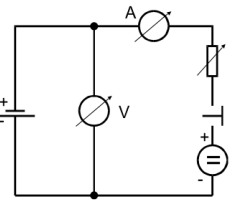
\includegraphics[scale=1.00]{abb2.png}
\caption{Versuchsaufbau mit Gegenspannung}
\label{Aufbau2}
\end{figure}Analog zu oben werden der f\"ur 11 verschiedene Lastwiderst\"ande von $0\,\Omega$ bis $100\,\Omega$ die Klemmenspannung und der flie\ss ende Strom gemessen. F\"ur die gemesssene Spannung gilt nun nach der Maschenregel
\begin{equation}
U_k = U_0 - U_g - I_*R.
\end{equation}
\section{Auswertung}


\subsection{Bestimmung von $U_0$ und $R_i$}
Zur Bestimmung des Innenwiderstandes und der Leerlaufspannung werden die gemessenen Spannungswerte f\"ur $U_k$ gegen den Strom $I$ aufgetragen. Abbildung \ref{Plot1} zeigt den Verlauf f\"ur die Monozelle, Abbildung \ref{Plot2} f\"ur die Rechteckspannung und Abbildung \ref{Plot3} f\"ur die Sinusspannung. Alle Messwerttabellen des Versuches befinden sich im Anhang.


 

\begin{sidewaysfigure}[htp]
\centering
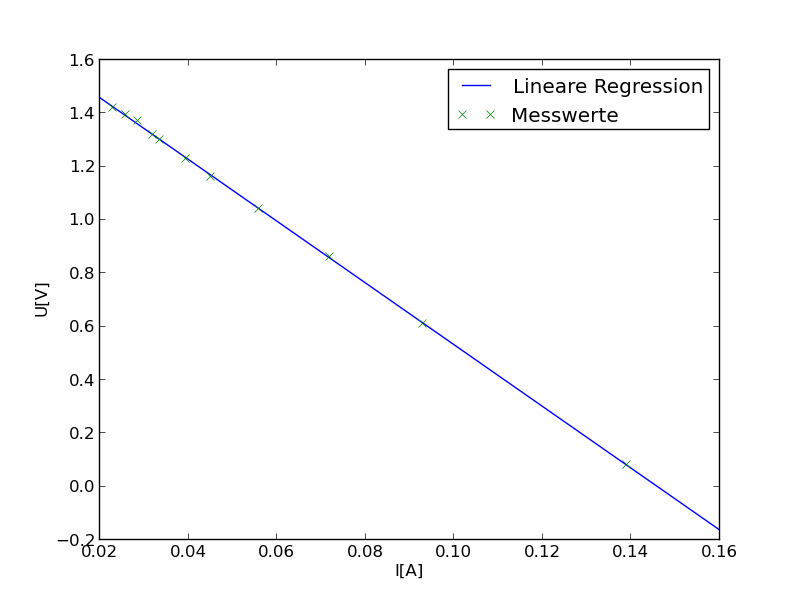
\includegraphics[scale=1.00]{Plot1.png}
\caption{$U_k$ in Abh\"angigkeit von $I$ f\"ur die Monozelle}
\label{Plot1}
\end{sidewaysfigure}

\begin{sidewaysfigure}[htp]
\centering
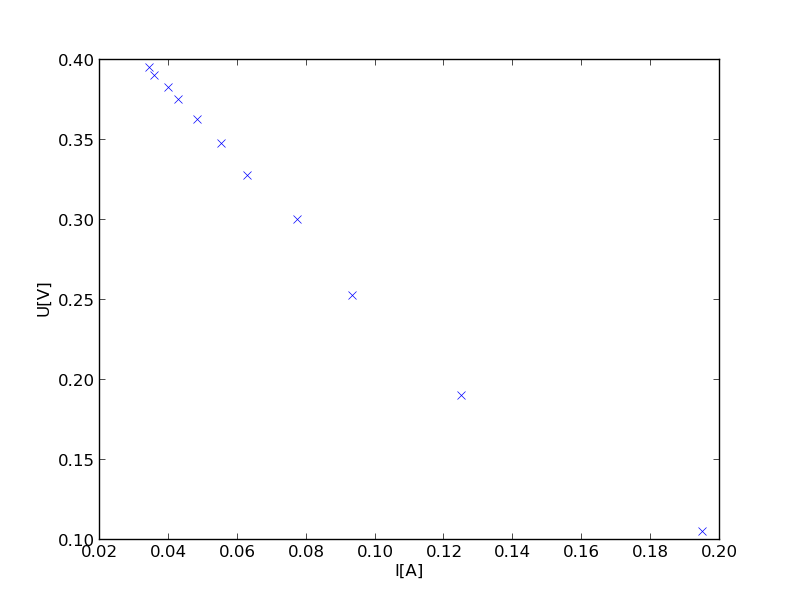
\includegraphics[scale=1.00]{Plot2.png}
\caption{$U_k$ in Abh\"angigkeit von $I$ f\"ur die Monozelle}
\label{Plot2}
\end{sidewaysfigure}
\begin{sidewaysfigure}[htp]
\centering
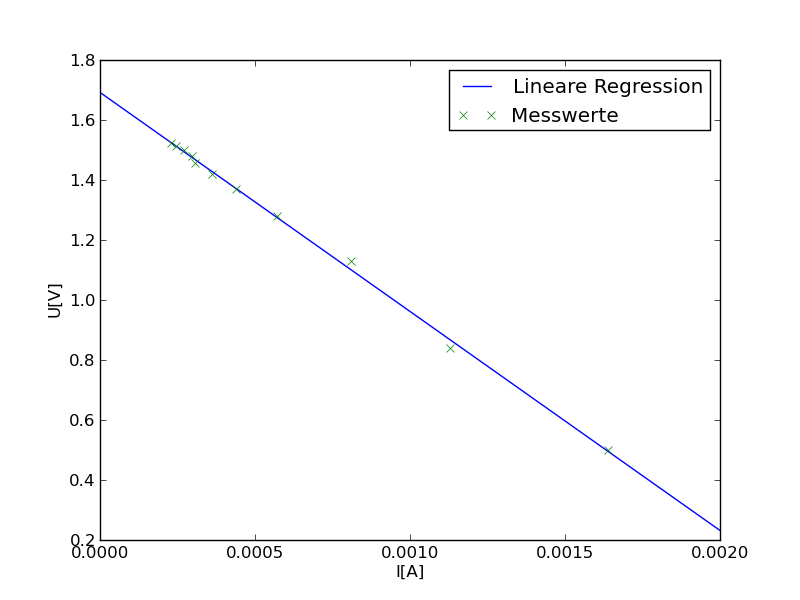
\includegraphics[scale=1.00]{Plot3.png}
\caption{$U_k$ in Abh\"angigkeit von $I$ f\"ur die Monozelle}
\label{Plot3}
\end{sidewaysfigure}
\newpage
\noindent
Mit Hilfe der Linearen Regression können jeweils der Innenwiderstand und die Leerlaufspannung der Spannungsquellen bestimmt werden. Folgende Werte wurden mit Python ermittelt:

 \begin{table}[h]
 \centering
 \caption{Ergebnis}
 \begin{tabular}{|c|c|c|}
  \hline
  Spannungsquelle & $R_I[\Omega]$ & $U[V]$ \\
  \hline
  Monozelle & $(11.58\pm$0.05) & $(1.6899\pm0.0028)$ \\
  Rechteckspannung & $(61.3\pm0.9)$& $(0.4823\pm0.0028)$ \\
  Sinusspannung & $(730\pm10)$ & $(1.692\pm0.007)$\\
  \hline
 \end{tabular}
 \label{Ergebnis}
 \end{table}

\subsection{Direkte Messung von $U_0$}
Die direkte Messung von $U_0$ der Monozelle ergab eine Leerlaufspannung von $1.68\, V$. Der Fehler der Leerlaufspannung ergibt sich aus einer kurzen Herleitung:\newline
Aus Formel (3) ergibt sich
\[ U_0 = U_k + I \cdot R_v. \]
Mit $I=U_k / R_v$ ist
\[ U_0 = U_k + \frac{U_k \cdot R_i}{R_v}.\]
Durch Ausklammern von $U_k$ erhält man
\[ U_0 = U_k \left( 1+\frac{R_i}{R_v}\right) .\]
Nun ergibt sich der Fehler der Leerlaufspannung als
\[ \Delta U = \frac{U_k \cdot R_i}{R_v}. \]
Der Fehler der Leerlaufspannung der Monozelle beträgt jetzt
\[ \Delta U_0 = 1.946 \cdot 10^{-6}.\]
\newline
Falls man das Voltmeter für die Messung der Spannung in der Schaltung hinter das Amperemeter setzt, macht man systematische Fehler. So zeigt eine Betrachtung der Maschenregel
\[ 0 = -U_0 + U_k + R_i \cdot I + R_{Amp} \cdot I ,\]
dass an dem Amperemeter auch ein Teil der Spannung abfällt:
\[ U_k = U_0 - I(R_i + R_{Amp}). \]
\newline
Die mit dem Voltmeter gemessene Leerlaufspannung wird daher kleiner.
\subsection{Leistung der Monozelle}

\section{Diskussion}
Die Multimeter haben eine Messgenauigkeit von $\pm 3 \%$. Die Multimeter sind allerdings analog, bei der Messung der RC-Generatoren waren die Zeiger teilweise in Schwingung. Dadurch ergibt sich eine Messungenauigkeit durch das Ablesen der Messwerte. Der angegebene Fehler von $\pm 3 \%$ kann daher vernachlässigt werden.
 
\section{Abbildungsverzeichnis}
\begin{itemize}
\item Abbildung 1,2 und 3: Versuch 301 \textit{Leerlaufspannung und Innenwiderstand von Spannungsquellen}, Physikalisches Praktikum\\ TU Dortmund
\end{itemize}
\section{Anhang}
\begin{table}[h]
 \centering
 \caption{Messung an der Monozelle}
 \begin{tabular}{|c|c|}
  \hline
  $U[V]$ & $I[mA]$  \\
  \hline
  1.42 & 23 \\
  1.395 & 25.9 \\
  1.37& 28.5 \\
  1.32 & 31.9 \\
  1.30 & 33.5\\
  1.23 & 39.5\\
  1.16 & 45 \\
  1.04 & 56\\
  0.86 & 72\\
  0.61 & 93\\
  0.082 & 139\\
  \hline
 \end{tabular}
 \label{Messung 1}
 \end{table}
 
 
 \begin{table}[h]
 \centering
 \caption{Messung an der Monozelle mit Gegenspannung}
 \begin{tabular}{|c|c|}
  \hline
  $U[V]$ & $I[mA]$  \\
  \hline
  2.07 & 34.5 \\
  2.09 & 36 \\
  2.15 & 40 \\
  2.19 & 43 \\
  2.26 & 48.5\\
  2.35 & 55.5\\
  2.42 & 63 \\
  2.58 & 77.5\\
  2.718 & 93.5\\
  2.91 & 125\\
  3.73 & 195\\
  \hline
 \end{tabular}
 \label{Messung 2}
 \end{table}
 
 
 \begin{table}[h]
 \centering
 \caption{Messung an der Rechteckspannung}
 \begin{tabular}{|c|c|}
  \hline
  $U[V]$ & $I[mA]$  \\
  \hline
  0.395 & 1.4 \\
  0.39 & 1.46 \\
  0.3825& 1.61 \\
  0.375 & 1.75 \\
  0.3625 & 1.97\\
  0.3475 & 2.25\\
  0.3275 & 2.62 \\
  0.3 & 3.05\\
  0.2525 & 3.6\\
  0.19 & 4.7\\
  0.105 & 6.2\\
  \hline
 \end{tabular}
 \label{Messung 3}
 \end{table}
 
 
 \begin{table}[h]
 \centering
 \caption{Messung an der Sinusspannung}
 \begin{tabular}{|c|c|}
  \hline
  $U[V]$ & $I[mA]$  \\
  \hline
  1.525 & 0.23 \\
  1.5125 & 0.245 \\
  1.5& 0.2725 \\
  1.48 & 0.296 \\
  1.455 & 0.305\\
  1.42& 0.361\\
  1.37 & 0.44 \\
  1.28 & 0.57\\
  1.13 & 0.81\\
  0.84 & 1.13\\
  0.5 & 1.64\\
  \hline
 \end{tabular}
 \label{Messung 4}
 \end{table}

\end{document}
